\documentclass{MetricNotes2023}

\usepackage[a4paper,top=2cm,bottom=2cm,left=2cm,right=2cm,marginparwidth=1.75cm]{geometry}

\usepackage{graphicx}
\graphicspath{ {./images/} }
\usepackage{float}

%inserting a figure:

%\begin{figure}[h]
%\centering
%\includegraphics[width=0.5\textwidth]{pfigure_1}
%\caption{The compound pendulum}
%\end{figure}
%\setcounter{MaxMatrixCols}{20}
\usepackage{amsmath}
\usepackage{enumitem}
\usepackage{amssymb}
\usepackage{amsthm}
\usepackage[colorlinks=true, allcolors=blue]{hyperref}
\usepackage{mathtools}
\usepackage{parskip}
\usepackage{mathrsfs}
\usepackage{float}

% knots stuff

\usepackage{tikz}
\usetikzlibrary{cd}
\usetikzlibrary{shapes,snakes}
\usepackage{listings}

%\graphicspath{ {figs/} }

\usepackage{cleveref}
\newcommand{\notimplies}{%
  \mathrel{{\ooalign{\hidewidth$\not\phantom{=}$\hidewidth\cr$\implies$}}}}

%keyword: edit

\newcommand{\surj}{\rightarrow\mathrel{\mkern-14mu}\rightarrow}

\newcommand{\xsurj}[2][]{%
  \xrightarrow[#1]{#2}\mathrel{\mkern-14mu}\rightarrow
}

\newcommand\xmono[2][]{\ensurestackMath{\mathrel{%
  \stackengine{1pt}{%
    \stackengine{0pt}{\rightarrowtail}{\scriptstyle#2}{O}{c}{F}{F}{S}%
  }{\scriptstyle#1}{U}{c}{F}{F}{S}%
}}}

\def\bb{\ensuremath\mathbb}
\def\la{\ensuremath\langle}
\def\ra{\ensuremath\rangle}
\def\notto{\ensuremath\nrightarrow}
\def\subq{\ensuremath\subseteq}
\def\inj{\ensuremath\hookrightarrow}
\def\xinj{\ensuremath\xhookrightarrow}
\def\comp{\ensuremath\mathbb{C}}
\def\real{\ensuremath\mathbb{R}}
\def\rat{\ensuremath\mathbb{Q}}
\def\inte{\ensuremath\mathbb{Z}}
\def\nat{\ensuremath\mathbb{N}}
\def\topo{\ensuremath\mathcal{T}}
\def\del{\ensuremath\partial}
\def\SIgma{\ensuremath\Sigma}

\def\A{\ensuremath{\mathscr{A}_2}}

\def\sequiv{\ensuremath\stackrel{\text{S}}{\sim}}
\def\rr{\ensuremath\mathcal{R}}
\def\com{\ensuremath\Delta}
\def\id{\ensuremath\text{id}}
\def\hopf{\ensuremath\mathcal{H}}

\DeclareMathOperator{\Arg}{Arg}
\DeclareMathOperator{\can}{can}
\DeclareMathOperator{\charr}{char}
\DeclareMathOperator{\cod}{cod}
\DeclareMathOperator{\coev}{coev}
\DeclareMathOperator{\coker}{coker}
\DeclareMathOperator{\colim}{colim}
\DeclareMathOperator{\dom}{dom}
\DeclareMathOperator{\End}{End}
\DeclareMathOperator{\ev}{ev}
\DeclareMathOperator{\Ext}{Ext}
\DeclareMathOperator{\Fix}{Fix}
\DeclareMathOperator{\Frac}{Frac}
\DeclareMathOperator{\Gr}{Gr}
\DeclareMathOperator{\Hom}{Hom}
\DeclareMathOperator{\im}{im}
\DeclareMathOperator{\lk}{lk}
\DeclareMathOperator{\mor}{mor}
\DeclareMathOperator{\ob}{ob}
\DeclareMathOperator{\Open}{Open}
\DeclareMathOperator{\Rep}{Rep}
\DeclareMathOperator{\Sk}{Sk}
\DeclareMathOperator{\Spec}{Spec}
\DeclareMathOperator{\SPec}{Spec}
\DeclareMathOperator{\str}{str}
\DeclareMathOperator{\tr}{tr}
\DeclareMathOperator{\trace}{trace}
\DeclareMathOperator{\cvec}{Vec}

\def\done{\begin{flushright}\vspace{-4.35ex}\(\qed\)\end{flushright}}

\DeclareSymbolFont{bbold}{U}{bbold}{m}{n}
\DeclareSymbolFontAlphabet{\mathbbold}{bbold}

% \limits\sum or \sum\limits (one of them) will put the text under the sum
% [upquote=true] on \begin{lstlisting} will stop backticks being interpreted as quotes
%[backend=bibtex, style=ieee]
\usepackage[backend=bibtex]{biblatex}
%\bibliographystyle{plain}
%\usepackage{csquotes}
\addbibresource{References.bib}

\author{\vspace{-5ex}}
%\title{Something True and Beautiful [DRAFT]}
\title{Stable Homotopy Groups of Spheres  [DRAFT]}
\date{\vspace{-5ex}}

\counterwithin{figure}{section}

\begin{document}
\maketitle
%\input{titlepage.tex}

\DeclarePairedDelimiter{\norm}{\lVert}{\rVert} 
\DeclarePairedDelimiter{\abs}{\lvert}{\rvert} 
\DeclarePairedDelimiter{\ang}{\langle}{\rangle} 

\tableofcontents

\pagebreak

\section{Introduction}

\begin{itemize}
\item Define homotopy groups
\item Freudenthal's suspension theorem: if \(\pi_i(X)=0\) for \(i\leq k\) (i.e. \(X\) is \(k\)-connected) then the map 
\begin{align*}
\pi_n(X) \;\;&\to\;\; \pi_{n+1}(\Sigma X)\\
[\gamma : S^n \to X] &\mapsto [\Sigma \gamma : \Sigma S^n=S^{n+1} \to \Sigma X]
\end{align*}
is an isomorphism for \(n \leq 2k\) and surjective for \(n=2k+1\)
\item This implies \(\pi_{n+k}(S^n)\) depends only on \(k\) for \(n\geq k+2\)
\item (Obviously be careful with basepoints above)
\item Suppose \(X\) is \(k\)-connected. Then, for \(k\geq 0\), \(0=\pi_k(X)\cong \pi_{k+1}(\Sigma X)\), so whenever a space is \(k\)-connected its suspension is \(k+1\)-connected. 
\item As you take suspensions, then, your successive bounds are \(n \leq 2k\), \(n+1\leq 2k+2\implies n \leq 2k+1\), \(n\leq 2k+2\), etc ... so the sequence \(\pi_n(X)\to \pi_{n+1}(\Sigma X)\to \cdots\) will eventually stabilise.  
\item Thus, if you take the colimit of that direct system, it'll just equal the stable value, with the higher legs just being the inverse isomorphisms.
\item \autocite{ass}, Cor 1.9 [not 100\% convinced of how this follows, but believing it for now]: if \(X\) is a CW complex of dimension \(d\) and \(Y\) a \((k-1)\)-connected space, then the suspension homomorphism\footnote{Hang on, the what?? \(X\) isn't the suspension of anything, why on earth would this be a group?} \([X, Y]\to[\Sigma X, \Sigma Y]\) is bijective if \(d<2k-1\) and surjective if \(d=2k-1\). 
\end{itemize}

Miscellaneous facts I might need later:
\begin{itemize}
\item Cohomology [possibly only of pointed %\footnote{What's the relevance of the `pointedness' when you're only taking cohomology?} %I think it's just that it's reduced
CW complexes] is representable\footnote{As a set, or is this some sort of enriched thing? If it's enriched, is that over \textbf{Ab} or \textbf{Rng}? \autocite{hatcher} says on p394 that there is a natural group structure on \(\Hom(X,K(G,n))\) such that the natural isomorphism \(\Hom(X,K(G,n))\to H^n(X;G)\) is in fact an isomorphism of abelian groups. So, it's over \textbf{Ab}? N.B: There's a lot of talk about `reduced cohomology theories', so a good next step would be to figure out what those are - if they only involve groups and not rings, maybe the cup product on \(H^*\) is not relevant here.}, and its representing object is the Eilenberg-MacLane space.  i.e. \(H^n(-; G)\cong \Hom(-, K(G, n))\). 
\item \(\mathscr A_2\) is generated as an algebra by elements \(Sq^{2^k}\) (\autocite{hatcher}, Prop 4L.8).
\item The map \(\mathscr A_2 \to \tilde H^*(K(\inte/2\inte, n); \inte/2\inte)\), \(Sq^I\mapsto Sq^I(\iota_n)\) is an isomorphism from the degree \(d\) part of \(\mathscr A_2\) onto \(H^{n+d}(K(\inte/2\inte, n); \inte/2\inte)\) for \(d \geq n\). In particular, the admissible monomials \(Sq^I\) form an additive basis for \(\mathscr A_2\). Thus, \(\mathscr A_2\) is exactly the algebra of all \(\inte/2\inte\) cohomology operations that are stable, commuting with suspension (\autocite{hatcher5}, Cor 5.38). 
\item ``Stable homotopy groups are a homology theory'' (whatever that means)
\item Hurewicz theorem: for any path-connected space \(X\) and \(n>0\) there exists a group homomorphism \(h_* : \pi_n(X)\to H_n(X)\). For \(n=1\) this induces an isomorphism \(\pi_1^{\text{ab}}(X)\cong H_1(X)\). For \(n \geq 2\), if \(X\) is \((n-1)\)-connected then \(\tilde H_i(X)=0\) for all \(i<n\), and the map \(h_* : \pi_n(X)\to H_n(X)\) is an isomorphism. 
\end{itemize}

\autocite{ass}, \autocite{suspension}, \autocite{hatcher}

\section{The Steenrod algebra}

The following is from \autocite{hatcher} 4L.

\begin{itemize}
\item There are maps \(Sq^i : H^n(-; \inte/2\inte)\to H^{n+i}(- ; \inte/2\inte)\) for each \(i\), and they satisfy the following properties: \begin{enumerate}
\item \(Sq^i_X(f^*(\alpha))=f^*(Sq^i_Y(\alpha))\) for \(f : X \to Y\) (i.e. \(Sq^i\) is a natural transformation).
\item \(Sq^i_X(\alpha + \beta)=Sq^i_X(\alpha)+Sq^i_X(\beta)\) (i.e. \(Sq_X^i\) respects the group operation for all \(X\)).
\item \(Sq^i(\alpha \smile \beta)=\sum\limits_{0\leq j \leq i} (Sq^j(\alpha)\smile Sq^{i-j}(\beta))\) (the Cartan formula)
\item \(Sq^i(\sigma(\alpha))=\sigma(Sq^i(\alpha))\) where \(\sigma : H^n(X; \inte/2\inte)\to H^{n+1}(\Sigma X; \inte/2\inte)\) is the ``suspension isomorphism given by reduced cross product with a generator of \(H^1(S^1; \inte/2\inte)\)''. [see: \autocite{hatcher}, p219. N.B: I think this ``relative cross product'' theory is required -- you can argue that there is an isomorphism via MV, but this point says that it's this specific one. Maybe they're the same, but Hatcher doesn't say that anywhere and there could be many isomorphisms.]
\item \(Sq^i(\alpha)=\alpha^2\) if \(i=\deg(\alpha)\) and \(Sq^i(\alpha)=0\) if \(i> \deg(\alpha)\). %[Hatcher doesn't explain this notation at all, but I think he means by \(\abs{\alpha}\) the degree of \(\alpha\) - this is what \autocite{stable_homotopy2} says in C2] N.B: I'm right, he defines in on p212 of AT
\item \(Sq^0=\id.\)
\item \(Sq^1\) is the ``\(\inte/2\inte\) Bockstein homomorphism \(\beta\) associated with the coefficient sequence \(0 \to \inte/2\inte \to \inte/4\inte \to \inte/2\inte \to 0\)''. 
\end{enumerate}
\item Define \(Sq:=Sq^0+Sq^1+\cdots\). Then \(Sq(\alpha\smile \beta)=Sq(\alpha)\smile Sq(\beta)\) (since \((Sq(\alpha\smile \beta))_n=\sum_iSq^i(\alpha)\smile Sq^{n-i}(\beta)=(Sq(\alpha)\smile Sq(\beta))_n\)). Thus, \(Sq\) is a ring homomorphism. 
\item Adem relations:
\[Sq^aSq^b=\sum_j {b-j-1\choose a-2j}Sq^{a+b-j}Sq^j \quad \text{if } a<2b,\]
where \({m \choose n}\) is zero if \(m\) or \(n\) is negative, or \(m<n\), and \({m \choose 0}=1\) for \(m \geq 0\).
\end{itemize}

\begin{definition}
The \textit{Steenrod algebra} \(\mathscr{A}_2\) is the algebra over \(\inte/2\inte\) that is the quotient of the algebra of polynomials in the noncommuting variables \(Sq^1, Sq^2, ...\) by the two-sided ideal generated by the Adem relations. Thus, for every space \(X\), \(H^*(X; \inte/2\inte)\) is a module over \(\mathscr A_2\).
\end{definition}

[When is \(H^*(X; \inte/2\inte)\) generated as an \(\A\)-module by only finitely many \(\alpha_i\) in each degree? If each \(H^i(X; \inte/2\inte)\) is finitely generated, then picking those generators would certainly work...]

\begin{itemize}
\item \(\mathscr A_2\) is graded, and its elements of degree \(k\) are those that map \(H^n(X; \inte/2\inte)\) to \(H^{n+k}(X, \inte/2\inte)\) for all \(n\). [Presumably you've fixed a space \(X\) while you're doing all this?]
\end{itemize}

\begin{definition}
Write \(Sq^I\) for the monomial \(Sq^{i_1}Sq^{i_2}\cdots Sq^{i_n}\). Then \(Sq^I\) is \textit{admissible} if \(i_j\geq 2i_{j+1}\) for all \(0\leq j < n\). 
\end{definition}

Note the admissible monomials are exactly those to which no Adem relations can be applied. Thus, \(\A\) is generated as a \(\inte/2\inte\) module by admissible monomials. 

\autocite{stable_homotopy}, \autocite{cobordism}, 
\autocite{ass}, \autocite{spectra}, \autocite{hatcher}, \autocite{foundations}

%\section{Spectra may not be your friends, but I can introduce you}
\section{Spectra}

\subsection{Categorical nonsense}

\begin{itemize}
\item \autocite{ass}: There is a category \(\mathcal{H}\) of finite %[because the corollary wanted f.d. CW complexes] 
based CW  complexes, with \(\Hom(X, Y)=:[X, Y]\) the set of homotopy classes of base-point preserving maps \(X\to Y\).
\item There is a category \textbf{St}(\(\mathcal{H}\)) of finite based CW complexes, with \(\Hom(X, Y)=:\{X, Y\}\) the  set \(\colim_i [\Sigma^iX, \Sigma^iY]\) [it's just a colimit of sets, and \textbf{Set} is cocomplete, so we should be fine. \autocite{ass} says it's a group\footnote{The colimit is equal to the stable value (which exists, by the corollary). After \(\Sigma^2\), these guys are all groups, so the colimit also has a group structure inherited from whatever \([\Sigma^k X, \Sigma^k Y]\) it's equal to. N.B: Remarks about cocompleteness of \textbf{Set} are misleading because that doesn't actually matter - any sequence that stabilises in any category will have a filtered colimit equal to that stable value, you don't need any extra conditions.}] [Also, how do these guys compose?]
\item There is a functor \(\mathcal{H}\to \textbf{St}(\mathcal{H})\). \autocite{ass} doesn't say what this is but it's presumably the one that is the identity on objects and sends \([f : X \to Y]\in [\Sigma^0X, \Sigma^0Y]\) to whatever it gets sent to in \(\{X, Y\}\) using the universal property of the colimit. Uniqueness makes it functorial, etc.
\item We have a fully faithful functor \(\textbf{St}(\mathcal{H})\to \textbf{St}(\mathcal{H})\) given by the suspension on objects, and the unique isomorphism \(\{X, Y\}\to\{\Sigma X, \Sigma Y\}\) on maps (such an isomorphism exists, since both of those things are colimits for \([\Sigma^i X, \Sigma^i Y]\) - one of the sequences is cut off at the beginning, but it doesn't matter because both reach the stable value (see above discussion and \autocite{ass} 1.9), aka the colimit). 
\item It's not an equivalence, because not every object is isomorphic to a suspension (e.g. anything not connected, since suspensions always connected [?])
\item We can formally adjoin desuspensions \(\Sigma^{-n}X\) for all \(n\) [does this mean just putting the objects there and defining \(\Hom(Y, \Sigma^{-n}X):=\Hom(\Sigma^nY, X)\) and \(\Hom(\Sigma^{-n}X, Y):=\Hom(X, \Sigma^n Y)\)?], but this category does not have weak colimits (i.e. colimits w/o uniqueness property). [why does it not, and why do we even want that?]
\item We instead consider formal sequences of desuspensions \(X_0 \to \Sigma^{-1}X_1 \to \cdots\), or sequences \((X_n)\) and maps \(\Sigma X_n \to X_{n+1}\), i.e. spectra. [and this fixes the problem?]
\end{itemize}

\subsection{Definitions and examples}

Below follows \autocite{hatcher5}, Section 
5.2.

[Maybe I could also look at \autocite{hatcher} p454 onwards?]

\begin{definition}
A \textit{spectrum} is a collection of pointed topological spaces \(\{X_n\}_{n\in \nat}\), together with basepoint-preserving maps \(\sigma_n : \Sigma X_n \to X_{n+1}\).
\end{definition}

\begin{example}
Let \(X\) be a topological space. The \textit{suspension spectrum} of \(X\), denoted by \(\Sigma^\infty X\), has \(X_n=\Sigma^nX\) and \(\sigma_n=\id : \Sigma X_n \to X_{n+1}\).
\end{example}

We write \(\bb{S}:=\Sigma^\infty S^0\), and call \(\bb{S}\) the \textit{sphere spectrum}. 

\begin{example}
The \textit{Eilenberg-MacLane spectrum} has \(X_n\) a CW complex \(K(G,n)\) and \(\sigma_n : \Sigma K(G,n)\to K(G,n+1)\) is the adjoint of the CW approximation \(K(G, n)\to \Omega K(G,n+1)\).
\end{example}

%[N.B. the important point of the above is not that it's `an' EM space rather than `the' (they're all homotopy equivalent). It's that a) we can definitely construct one that's a CW complex, and b) even though \(\Omega\)(a CW complex) is not necessarily a CW complex, we can make it one via CW approximation.]

\begin{definition}
Let \(X=\{X_n\}\) be a spectrum. We define \(\pi_i(X)=\colim_n \pi_{i+n}(X_n)\), where the map \(\pi_{i+n}(X_n)\to \pi_{i+n+1}(X_{n+1})\) is given by the composition
\[\pi_{i+n}(X_n)\xrightarrow{\Sigma}\pi_{i+n+1}(\Sigma X_n)\xrightarrow{(\sigma_n)_*}\pi_{i+n+1}(X_{n+1}).\]
\end{definition}

\begin{example}
If \(X\) is a topological space, then \(\pi_i(\Sigma^\infty X)=\pi_i^S(X)\), the \(i\)th stable homotopy group of \(X\). 
\end{example}

\begin{definition}
A CW spectrum is a spectrum \(X\) consisting of CW complexes \(X_n\) with the maps \(\Sigma X_n \inj X_{n+1}\) inclusions of subcomplexes. 
\end{definition}

\begin{definition}
Let \(X\) be a CW spectrum. Then the \textit{\(k\)-cells} of \(X\) are the equivalence classes of non-basepoint \(k+n\)-cells in \(X_n\), where two cells are equivalent if one is an \(m\)-fold suspension of the other. 
\end{definition}

%[Insert brief but enlightening observation of the effect of suspension on cells of CW complexes here]

%[\autocite{hatcher} says on p12 (god, way to make me feel stupid) that ``in \(\Sigma X\) there is a single 0-cell and an \((n+1)\)-cell for each \(n\)-cell of \(X\) other than [the basepoint]''.]

\begin{definition}
A CW spectrum \(X\) is \textit{connective} if it has no cells below a given dimension. Further, \(X\) is \textit{finite} if it has only finitely many cells, and \textit{of finite type} if it has only finitely many cells in each dimension.
\end{definition}

\begin{example}
If \(X\) is a finite (resp. finite type) CW complex, then \(\Sigma^\infty\) is a finite (resp. finite type) CW spectrum. In particular, \(\bb{S}\) is a finite CW spectrum with a unique cell in dimension 1.
\end{example}

\subsection{Homology and cohomology}

[From Hatcher: ``the inclusions \(\Sigma X_n \inj X_{n+1}\) induce inclusions \(C_*(X_n; G)\inj C_*(X_{n+1}; G)\) with a dimension shift to account for the suspension''. Below is my vague explanation of what I understand this to mean.

\(C_i(X_n; G)\) is the free abelian group on maps \(\Delta^i \to X_n\). I claim \(\Sigma\Delta^i\cong \Delta^{i+1}\). If this is true, it gives a map
\begin{align*}
C_i(X_n;G) &\to C_{i+1}(\Sigma X_n; G)\\
f &\mapsto \Sigma f.
\end{align*}
This is an injection, by \ref{2502141442}. We also have an injection \(C_{i+1}(\Sigma X_n; G)\to C_{i+1}(X_{n+1}; G)\) induced by the structure map \(\sigma_n\), so we get an injection \(C_i(X_n;G)\inj C_{i+1}(X_{n+1};G)\), which indeed has a dimension shift.

We then have that ``the union \(C_*(X ; G)\) of this increasing sequence of chain complexes is then a chain complex having one \(G\) summand for each cell of \(X\)''. I think that 
\[C_n(X ; G)=\bigcup_{i\in \inte}C_{i+n}(X_i; G),\] 
so that there's a \(G\) summand for every \(i+n\) cell of \(X_i\) up to treating suspensions of cells as equivalent to the cells themselves (since they include in), i.e. a \(G\) summand for every \(n\)-cell of \(X\), since that's how we defined them.

%Some issues:
%\begin{itemize}
%\item The way it's phrased, it seems to be that this is a morphism of chain complexes - i.e. these maps commute with the \(\del\)s. Why would they?]
%\end{itemize} I don't think so?

We define \(H^*\) and \(H_*\) to be the cohomology and homology of this chain complex, respectively.]

\begin{definition}
Let \(X=\{X_n\}\) be a CW spectrum. A \textit{subspectrum} \(X'\) of \(X\) is a sequence of subcomplexes \(\{X_n'\subq X_n\}\) satisfying \(\Sigma X_n'\subq X_{n+1}'\). The subspectrum \(X'\) is \textit{cofinal} if, for each \(n\) and each cell \(e^i_\alpha\) of \(X_n\), the cell \(\Sigma^k e_\alpha^i\) belongs to \(X'_{n+k}\) for all sufficiently large \(k\).
\end{definition}

[If \(\Sigma^ke^i_\alpha\) belongs to \(X'_{n+k}\) then \(\SIgma^{k+1}e^i_\alpha\) belongs to \(\Sigma X'_{n+k}\inj X'_{n+k+1}\), so if it happens once it'll happen for all time after that. Thus, if \(X'\), \(X''\) are cofinal spectra of \(X\) with \(\Sigma^k e_{\alpha}^i\) a cell of \(X_{n+k}'\) and \(\Sigma^l e_\alpha^i\) a cell of \(X_{n+l}''\) (\(l\geq k\)) then \(\Sigma^l e_\alpha^i\) is a cell of \(X_{n+l}'\) and therefore of \(X_{n+l}'\cap X_{n+l}''\). In other words, the intersection of two cofinal spectra is a cofinal spectrum.]

\begin{definition}
Let \(X, Y\) be CW spectra. A \textit{strict map} \(f : X \to Y\) is a sequence of cellular maps \(f_n : X_n \to Y_n\) such that the diagram below commutes.
\[\begin{tikzcd}
\Sigma X_n \arrow[r, "\sigma_n"] \arrow[d, swap, "\sigma f_n"]  & X_{n+1} \arrow[d, "f_{n+1}"]  \\
\SIgma Y_n \arrow[r, swap, "\sigma_n"]  & Y_{n+1}
\end{tikzcd}\]
\end{definition}

[this induces maps \(\pi_i(X)\to\pi_i(Y)\), \(H^*(Y)\to H^*(X)\), \(H_*(X)\to H_*(Y)\).]

\begin{definition}
A \textit{map} of CW spectra \(f : X \to Y\) is an equivalence class of strict maps \(f' : X' \to Y\) with \(X'\) a subspectrum of \(X\), where two strict maps \(f' : X' \to Y\) and \(f'' : X'' \to Y\) are equivalent if they agree on some common cofinal spectrum. 
\end{definition}

[this also induces maps \(\pi_i(X)\to\pi_i(Y)\), \(H^*(Y)\to H^*(X)\), \(H_*(X)\to H_*(Y)\).]

[check composition is well defined]

[working definition of equivalence below:]

\begin{definition}
Two spectra \(X, Y\) are \textit{equivalent} if there are maps \(f : X \to Y\) and \(g : Y \to X\) such that \(fg=\id_{Y}\) and \(gf=\id_X\).
\end{definition}

Note that a spectrum is equivalent to any of its cofinal subspectra.

[A spectrum is always equivalent to the suspension of some other spectrum]

%We say that two maps \(f, g : X \to Y\) of CW spectra are equivalent if they take the same value on some common cofinal spectrum, 

\begin{definition}
A \textit{homotopy} of maps between spectra is a map \(X\times I \to Y\), where \(X\times I\) is the spectrum with \((X\times I)_n=X_n\times_{\text{red}} I\).
\end{definition}

Note that \(\Sigma(X_n\times_{\text{red}}I)=\Sigma X_n\times_{\text{red}}I\). The set of homotopy classes of maps \(X\to Y\) is denoted by \([X,Y]\). 

\begin{remark}
For any CW spectra \(Z\), \([\Sigma^\infty S^t, Z]=\pi_t(Z)\). [they satisfy the same universal property]
\end{remark}

[\autocite{stable_homotopy} says on p171 that ``\([\Sigma X, Z]\) is obviously a group, because in \(\Sigma X\) we have a spare suspension coordinate out in front to manipulate. And for the same reason, \([\Sigma^2 X, Z]\) is an abelian group. But now we can give \([X,Y]\) the structure of an abelian group, because \([X,Y]\) is in 1-1 correspondence with \([\Sigma^2X, \Sigma^2 Y]\) and we pull back the group structure on that. So now our sets of morphisms \([X,Y]\) are abelian groups, and it's easy to see that composition is bilinear''. 

Various claims:
\begin{itemize}

%\item A spectrum is equivalent\footnote{Whatever that means.} to some suspension spectrum\footnote{Or probably just the suspension of a spectrum, see \ref{C}.}, so understanding \([X, Z]\) is the same as understanding \([\Sigma X, Z]\), which is the same as understanding \([\Sigma^2 X, Z]\). 
\item The stuff about normal CW complexes and their groups of maps (i.e. \ref{2502200937}) translates to tell me the appropriate things about spectra and their groups of maps.
\item After checking a lot of things, I can eventually conclude that \([X, Y]\) is an abelian group for spectra \(X, Y\).]
\end{itemize}

[The suspension map \([X,Y]\to[\Sigma X, \Sigma Y]\) is an isomorphism of groups]

[\ref{2502211419} and \ref{2502211420} are both true for CW spectra too]

[Whitehead's theorem: a map between CW spectra that induces isomorphisms on all homotopy groups is a homotopy equivalence.]

[Prop: If a CW spectrum \(X\) is \(n\)-connected in the sense that \(\pi_i(X)=0\) for \(i\leq n\), then \(X\) is homotopy equivalent to a CW spectrum with no cells of dimension \(\leq n\)]

\subsection{Cofibration sequences}

\begin{definition}
Let \(X=\{X_n\}, Y=\{Y_n\}\) be spectra. Then their \textit{wedge sum} %\footnote{This definition comes from \autocite{local}, but I'm a little suspicious because the nLab page says a wedge sum should always identify the basepoints, but the basepoint of a spectra surely isn't given by just a basepoint from each \(X_n\)? That's the only thing being identified here.} I think it's fine? just won't be an omega spectrum anymore, if that matters
 is \(X\vee Y :=\{X_n \vee Y_n\}\). Note that \ref{2502211505} gives us an inclusion \(\Sigma(X_n\vee Y_n)\inj X_{n+1}\vee Y_{n+1}\). 
\end{definition}

\begin{definition}
Let \(X\) be a spectrum, \(A\subq X\) a subspectrum. Then \(A\) is \textit{closed} in \(X\) if for every cell \(e_\alpha^n\) of \(X_n\), if \(\Sigma^k e_\alpha^n \in A_{n+k}\) then \(e_\alpha^n \in A_n\). 
\end{definition}

Note that any subspectrum is cofinal in (and thus equivalent to) its closure. We define \(X/A\) to be the CW spectrum with \((X/A)_n=X_n/A_n'\), where \(A'=\{A_n'\}\) is the closure of \(A\). 

[The rest of the section:

\begin{itemize}
\item Fact: for spectra \(X, Y\) and a subspectrum \(A\subq X\) we have exact sequences\footnote{Check if I actually need the first one.}
\[\cdots \to [\Sigma X, Y]\to [\Sigma A, Y]\to [X/A,Y]\to[X,Y]\to[A,Y]\]
\[[Y,A]\to[Y,X]\to[Y,X/A]\to[Y,\Sigma A]\to[Y,\Sigma X]\to\cdots\]
\end{itemize}

]

\autocite{stable_homotopy}, \autocite{cobordism}, \autocite{ass}, \autocite{spectra}, \autocite{foundations}, \autocite{hatcher5}

\section{The Adams spectral sequence}

\subsection{Spectral sequences}

[Maybe add some notes from \autocite{ass}]

[Some notes from \autocite{spectral_sequences}, C2 - just here as a placeholder/reference and I'll probably completely rewrite this bit.]

\begin{definition}
A \textit{differential bigraded module} \(E\) over a ring \(R\) is a collection of \(R\)-modules \(\{E^{p, q}\}\), \(p, q\in \inte\), together with a map \(d : E^{p, q} \to E^{p+s, q-s+1}\) for each \(p, q\) and some fixed \(s \in \inte\), satisfying \(d^2=0\). 
\end{definition}

We can take the homology of \((E, d)\):
\[H^{p, q}(E^{*, *}, d)=\ker(d : E^{p, q}\to E^{p+s, q-s+1})/\im(d : E^{p-s, q+s-1}\to E^{p, q}).\]

\begin{definition}
A \textit{spectral sequence} (of \textit{cohomological type}\footnote{I'll have to rewrite this section because the Adams spectral sequence is not a cohomological or a homological spectral sequence I don't think - the grading is \(d_r : E^{s,t}\to E^{s+r,t+r-1}\).}) is a collection of differential bigraded \(R\)-modules \(\{E^{*, *}_r, d_r\}, r \in \nat\), with the differentials \(d_r\) of bidegree \((r, 1-r)\). These satisfy the further condition that for all \(p, q, r\), \(E^{p, q}_{r+1}\cong H^{p, q}(E_r^{*, *}, d_r)\).
\end{definition}

We will sometimes write \(d^{p, q}_r\) for the differential \(d_r : E^{p, q}\to E^{p+r,q-s+1}\). 

Consider the term \(E_2^{*, *}\). Define 
\[Z_2^{p, q}:=\ker d_2^{p,q} \quad \text{and} \quad B_2^{p,q}:=\im d_2^{p-2,q+1}.\]
The condition \(d^2=0\) implies that \(B_2^{p,q}\subq Z_2^{p,q}\subq E_2^{p,q}\), and by definition we have \(E_3^{p,q}\cong Z^{p,q}_2/B_2^{p,q}\). 

Now, write 
\[Z_3^{p, q}:=\ker d_3^{p,q} \quad \text{and} \quad B_3^{p,q}:=\im d_3^{p-3,q+2}.\]
Since \(Z_3^{p,q}\subq E^{p,q}_3\), it can be written as \(\overline{Z}_3^{p,q}/B_2^{p,q}\) for some \(\overline{Z}_3^{p,q}\subq Z_2^{p,q}\). Similarly, \(B_3^{p,q}\cong \overline B_3^{p,q}/B_2^{p,q}\) for some \(\overline B_3^{p,q}\subq Z_2^{p,q}\). Thus,
\[E_4^{p,q}\cong Z_3^{p,q}/B_3^{p,q}\cong \frac{\overline Z_2^{p,q}/B_2^{p,q}}{\overline B_3^{p,q}/B_2^{p,q}}\cong \overline Z_3^{p,q}/\overline B_3^{p,q}.\]

Iterating this process, we present the spectral sequence as an infinite tower of submodules of \(E_2^{p,q}\):
\[B_2^{p,q}\subq \overline B_3^{p,q}\subq \cdots \subq \overline B_n^{p,q}\subq \cdots \subq \overline Z_n^{p,q}\subq \cdots \subq \overline Z_3^{p,q}\subq Z_2^{p,q}\subq E_2^{p,q},\]
with the property that \(E^{p,q}_{n+1}\cong \overline Z_n^{p,q}/\overline B_n^{p,q}\). The differential \(d_{n+1}^{p,q}\) can be taken as a map \(\overline Z^{p,q}_n/\overline B_n^{p,q}\to\overline Z_n^{p,q}/\overline B_n^{p,q}\) with kernel \(\overline Z_{n+1}^{p,q}/\overline B_n^{p,q}\) and image \(\overline B_{n+1}^{p,q}\). The short exact sequence induced by \(d_{n+1}\),
\[0 \to \overline Z^{p,q}_{n+1}/\overline B_n^{p,q}\to \overline Z_n^{p,q}/\overline B_n^{p,q} \xrightarrow{d_{n+1}^{p,q}} \overline B_{n+1}^{p,q}/\overline{B}_n^{p,q}\to 0,\]
gives rise to isomorphisms \(\overline{Z}_n^{p,q}/\overline{Z}_{n+1}^{p,q}\cong \overline{B}_{n+1}^{p,q}/\overline{B}_n ^{p,q}\) for all \(n\). Conversely, a tower of submodules of \(E_2\), together with a set of isomorphisms, gives rise to a spectral sequence. 

\begin{definition}
An element of \(E_2^{p,q}\) \textit{survives to the \(r\)th stage} if lies in \(\overline{Z}_r^{p,q}\), having been in the kernel of the previous \(r-2\) differentials, and is \textit{bounded by the \(r\)th stage} if it lies in \(\overline{B}_r^{p,q}\). The bigraded module \(E_r^{*,*}\) is called the \textit{\(E_r\)-term} of the spectral sequence. 
\end{definition}

We define 
\[Z_\infty^{p,q}:= \bigcap_n \overline{Z}^{p,q}_n, \quad B_\infty^{p,q}:=\bigcup^n \overline{B}^{p,q}_n.\]
From the tower of inclusions, we see that \(B_\infty^{p,q}\subq Z^{p,q}_\infty\), so we define \(E_\infty^{p,q}:=Z_\infty^{p,q}/B_\infty^{p,q}\). 

\begin{definition}
A spectral sequence \textit{collapses at the \(N\)th term} if the differentials \(d_r^{p,q}=0\) for \(r\geq N\). 
\end{definition}

From the short exact sequence 
\[0 \to \overline Z^{p,q}_{r}/\overline B_{r-1}^{p,q}\to \overline Z_{r-1}^{p,q}/\overline B_{r-1}^{p,q} \xrightarrow{d_{r}^{p,q}} \overline B_{r}^{p,q}/\overline{B}_{r-1}^{p,q}\to 0,\]
the condition \(d_r^{p,q}\) forces  \(\overline{Z}^{p,q}_r=\overline{Z}_{r-1}^{p,q}\) and \(\overline{B}^{p,q}_r=\overline{B}_{r-1}^{p,q}\). The tower of submodules becomes
\[B_2^{p,q}\subq \overline B_3^{p,q}\subq \cdots \subq \overline B_{N-1}^{p,q}=B_N^{p,q}= \cdots=B_\infty^{p,q} \subq Z_\infty^{p,q}= \cdots = \overline Z_N^{p,q}=\overline Z^{p,q}_{N-1}\subq \cdots \subq \overline Z_3^{p,q}\subq Z_2^{p,q}\subq E_2^{p,q}.\]
Thus, \(E_\infty^{p,q}=E_N^{p,q}\). 

\subsection{Exact couples}

(Following \autocite{spectral_sequences}, C2)

\begin{definition}
Let \(D, E\) be \(R\)-modules, and let \(i : D \to D\), \(j : D\to E\), \(k : E \to D\) be module homomorphisms. We call \(\mathcal{C}=\{D, E, i, j, k\}\) an \textit{exact couple} if the diagram below is exact.
\[\begin{tikzcd}
 D \arrow[rr, "i"] && D \arrow[dl, "j"] \\ 
  & E \arrow[ul, "k"] &  
 \end{tikzcd}\] 
\end{definition}

Let \(d:=jk\), and define the following:
\begin{align*}
E'&:=H(E, d)=\ker d/\im d\\
D'&:=i(D)=\ker j\\
i'&:=i|_{i(D)} : D'\to D'\\
j'&:=i(x)\mapsto j(x)+dE : D'\to E'\\
k'&:=(e+dE)\mapsto k(e) : E' \to D'
\end{align*}

We call \(\mathcal{C}'=\{D', E'. i', j', k'\}\) the \textit{derived couple} of \(\mathcal{C}\). 

\begin{proposition}[\autocite{spectral_sequences}, Prop 2.7]
If \(\mathcal{C}=\{D, E, i, j, k\}\) is an exact couple, then \(\mathcal{C}'\) is also an exact couple.
\end{proposition}

\begin{theorem}[{\autocite{spectral_sequences}, Thm 2.8}]
Suppose \(D^{*,*}=\{D^{p,q}\}\) and \(E^{*,*}=\{E^{p,q}\}\) are bigraded modules equipped with homomorphisms \(i\) of bidegree \((-1,1)\)\footnote{This is the wrong index. For my purposes it should be \((-1, -1)\). So, the spectral sequence will not be of cohomological type, but hopefully the proof still goes through.}, \(j\) of bidegree \((0,0)\), and \(k\) of bidegree \((1,0)\), such that \(\{D^{*,*}, E^{*,*}, i, j, k\}\) is an exact couple. Then these data determine a spectral sequence \(\{E_r, d_r\}\) for \(r\in \inte_+\) of cohomological type, with \(E_r=(E^{*,*})^{(r-1)}\), the \((r-1)\)st derived module of \(E^{*,*}\) and \(d_r=j^{(r)}\circ k^{(r)}\). 
\end{theorem}

A bigraded exact couple may be displayed in the following diagram, known as a \textit{staircase diagram}:

\[\begin{tikzcd} 
   &  \vdots \arrow[d, "i"] &  & \vdots \arrow[d, "i"] & \\
 \cdots \arrow[r, "k"] & D^{p+2, q-1} \arrow[d, "i"] \arrow[r, "j"] & E^{p+2,q-1}  \arrow[r, "k"] & D^{p+3,q-1} \arrow[d, "i"] \arrow[r, "j"] & \cdots \\
 \cdots \arrow[r, "k"] & D^{p+1,q} \arrow[d, "i"] \arrow[r, "j"] & E^{p+1,q}  \arrow[r, "k"] & D^{p+2,q} \arrow[d, "i"] \arrow[r, "j"] & \cdots \\
 \cdots \arrow[r, "k"] & D^{p,q+1}  \arrow[d, "i"] \arrow[r, "j"] & E^{p,q+1}  \arrow[r, "k"] & D^{p+1,q+1} \arrow[d, "i"] \arrow[r, "j"] & \cdots \\
 & \vdots &  & \vdots & 
\end{tikzcd}\]

[This is the same staircase diagram that Hatcher is talking about (set \(D^{*,*}=\pi_*^SX_*\) and \(E^{*,*}=\pi_*K_*\)) - just modulo some tweak of \(i\)'s bigrading because the bigrading is a bit weird in the Adams spectral sequence.]

\subsection{The Adams spectral sequence}

Things I need before I can set it up (according to Hatcher \autocite{hatcher5}):

Let \(X\) be a CW spectrum of finite type.

\begin{itemize}
%\item Def: \(H^*(X)\).
%\item Def: A wedge of spectra (Hatcher doesn't trouble himself with defining this)
\item Fact: \(H^*(X)\) is finitely generated.
\item Fact: \(H^*(X)\) is an \(\mathscr{A}_2\)-module. [We know that's true for a topological space]
\item Fact: We can pick generators \(\alpha_i\) for \(H^*(X)\) as an \(\mathscr{A}_2\)-module such that there are at most finitely many in each \(H^n(X)\).
\item Fact: There \(\alpha_i\) determine a map \(X \to K_0\), where \(K_0\) is a wedge of EM spectra, and \(K_0\) has finite type. [the first part probably follows from the fact that \(H^m(X; G)\cong [X, K(G,m)]\) naturally in \(m\) and \(X\).]
\item Fact: We can replace that map with an inclusion [maybe via a mapping cylinder? What does Hatcher mean by replace - does he mean that the new map is homotopy equivalent to the old one?].
\item Fact: A quotient of connective spectra of finite type is again a connective spectrum of finite type.
\item Prop: \autocite{hatcher5}, 5.46.
%\item Def: The functor \(\pi^Y_t(Z)=[\Sigma^tY, Z]\) for a finite spectrum \(Y\).
\item Def: A cofibration. [see : \autocite{hatcher}, p398.]
\item Fact: If \(Z\) is a connective spectrum of finite type, then \(\pi_t(Z)\) is finitely generated.
%\item Fact: I can do this. I have all the necessary skills to pull this off. 
%\item Fact: I'm going to stop listing things I need to do and start actually doing them.
\end{itemize}

[\autocite{hatcher5} Thm 5.47 says that there is a spectral sequence \(\{E_r, d_r\}\) such that \(E_2^{s,t}=\Ext_{\mathscr{A}_2}(H^*(\bb{S}), H^*(\bb{S}))\), and \(\{E_r, d_r\}\implies \pi^S_*\) modulo any odd torsion.

At the bottom of p592 of \autocite{hatcher5}, it's mentioned that for a spectrum \(X\) of finite type, \(H^i(X)\cong \lim\limits_{\leftarrow n}H^{i+n}(X_n)\) as \(\mathscr{A}_2\)-modules. Thus, since \(\bb{S}\) is of finite type (it is actually finite), we have
\begin{align*}
H^i(\bb{S}; \inte/2\inte)&=\lim\limits_{\leftarrow n}H^{i+n}(S^n; \inte/2\inte)\\
&=\begin{cases}
\inte/2\inte & i = 0,\\
0 & \text{otherwise.}
\end{cases}
\end{align*}
(since they're all just either \(0\) or \(\inte/2\inte\), at least eventually). So, \(H^*(\bb{S})=\inte/2\inte\) in degree zero and nothing else.]

\begin{theorem}[{\autocite{hatcher5}, Thm 5.47}]
There is a spectral sequence \(\{E_r, d_r\}\) such that \(E_2^{s,t}=\Ext_{\A}^{s,t}(\bb{F}_2, \bb{F}_2)\) and \(\{E_r, d_r\}\implies \pi_*^S\) modulo torsion of odd order. 
\end{theorem}



\autocite{spectral_sequences}, \autocite{stable_homotopy}, \autocite{cobordism}, \autocite{foundations}, \autocite{hatcher5}, \autocite{ass}, \autocite{primer}

\subsection{Multiplicative structure}

[Rough sketch, details to fill in once I have the shape of things:

Fact: there is a multiplication 
\[E^{s,t}_2\otimes E^{s',t'}_2\to E^{s+s', t+t'}_2,\]
i.e. 
\[F^{s,t}/F^{s+1, t+1}\otimes F^{s',t'}/F^{s'+1, t'+1}\to F^{s+s', t+t'}/F^{s+s'+1, t+t'+1}.\]

And it satisfies the Leibniz rule, and it converges to the composition product on \(\text{}_2\pi_*^S\). 

Using \ref{2503171645shutupitsbeenalongterm} (which comes later but whatever, I'll reorder things), we get \(E_2^{s,t}=\Hom^t_{\A}(F_s, \bb{F}_2)\). So, if we have a minimal free resolution 
\[\cdots \to F_2 \to F_1 \to F_0 \to \bb{F}_2\]
of \(\bb{F}_2\) as an \(\A\)-module, and we have \(f \in \Hom^t_{\A}(F_s, \bb{F}_2), g \in \Hom^{t'}_{\A}(F_{s'}, \bb{F}_2)\), we multiply them as follows:

First, we put these resolutions side by side.
\[\begin{tikzcd}
F_{s+s'} \arrow[r, dashrightarrow,""] \arrow[d, swap, ""]  & F_{s'}[t]  \arrow[d, ""] \arrow[r, "g"] & \bb{F}_2[t+t']  \\
F_{s+s'-1} \arrow[r, dashrightarrow, ""] \arrow[d, ""] & F_{s'-1}[t] \arrow[d, ""] & \\
\vdots \arrow[d, ""] & \vdots \arrow[d, ""] &   \\
F_s \arrow[r, dashrightarrow, ""] \arrow[d, ""] \arrow[rd, "f"'] & F_0[t]  \arrow[d, twoheadrightarrow, ""] &   \\ 
F_{s-1} \arrow[d] & \bb{F}_2[t] & \\
\vdots \arrow[d] & & \\
F_0  \arrow[d] & & \\
\bb{F}_2 & & 
\end{tikzcd}\]
(The \([t]\) means shifted by \(t\) i.e. in degree \(t\) because the maps are.)

Then we inductively fill in the dotted arrows from the bottom up. So you can fill the first one because the modules are all free so you just need to say where the generator goes (a priori maybe there are infinitely many generators but it's ok because these are degree \(t\) maps and there are only finitely many in each degree), and the right map is surjective, so just do it the way you would do it. Likewise for the higher ones. 

This thing is hopefully well-defined.

A few other things:
\begin{enumerate}
\item We know that \(\pi_0^S=\inte\) since \(\pi_1S^1=\inte\) and \(n=1\leq 2=2(1)\), so this lies in the stable region. Now, \(E^{s,t}\) is actually supposed to converge to the associated graded of \(\inte_2\) (i.e. the 2-adics) I think? But either way, we know that for our filtration all the quotients are \(\inte/2\inte\). I claim\footnote{Here is an absolutely ridiculous argument for that: \((\inte_2, +)\) is a topological group. For any subgroup \(H\) of finite index \(n=2^km\), \(H\) is open (since by Lagrange's theorem \(n\inte_2\subq H\) and thus \(n\inte_2=2^k\inte_2\), so \(x+2^k\inte_2\) is an open ball around any \(x\in H\)). Now, every open subgroup of \(\inte_2\) is also closed (since it's complement is a union of open cosets), and it's apparently the case [elaborate] that the closed subgroups of \(\inte_2\) are the ideals \(2^k\inte_2\). These facts then imply that the filtration I give is the only possible one.} then that the filtration must be \(\cdots 4\inte_2 \subq 2\inte_2 \subq \inte_2\). 
\item If that's true then \(\iota=[1]\in \inte_2/2\inte_2\), and using the multiplication above we see \(\iota\) is a unit. We also have \(h_0=[2]\in 2\inte_2/4\inte_2\) so \(h_0=[2]=[2[1]]=[2\iota]\), so \(h_0\) acts on \(\iota\) by multiplication by 2.
\item Now, for any \(\kappa\in E^{s,t}_2\), \(h_0\cdot \kappa = (\iota h_0)\cdot \kappa=2\kappa\). 
\end{enumerate}
The notation's a bit weird above, when I say `multiplication by 2' I mean: take \(\kappa \in E^{s,t}=F^{s,t}/F^{s+1,t+1}\). Then \(2\kappa \in F^{s+1,t+1}\) since it's a bunch of \(\bb{F}_2\)'s. Take it's equivalence class to get an element of \(F^{s+1, t+1}/F^{s+2,t+2}\). That's what I really mean by \(2\kappa\) and it's in \(E^{s+1,t+1}\).

All this is to say if I start multiplying higher things by \(h_0\), that \textit{is} multiplying by 2. So I can start resolving extensions this way.]

\autocite{ass}

\section{Calculating stable homotopy groups}

\subsection{The \(E_2\) page}


\begin{lemma}[{\autocite{hatcher5}, Lem 5.49}]\label{2503171645shutupitsbeenalongterm}
For a minimal free resolution 
\[\cdots \to F_2 \to F_1 \to F_0 \to \bb{F}_2 \to 0\]
of \(\bb{F}_2=H^*(\bb{S})\) as an \(\A\)-module, we have \(\Ext_{\A}^{s,t}(\bb{F}_2, \bb{F}_2)=\Hom^t_{\A}(F_s, \bb{F}_2)\), where \(\Hom^t_{\A}(F_s, \bb{F}_2)\subq \Hom_{\A}(F_s, \bb{F}_2)\) consists of the morphisms which lower the degree by \(t\).
\end{lemma}

[Now, since \(\bb{F}_2\) just has stuff in degree 0, the only things that can be sent to \(1 \in \bb{F}_2\) are the things in degree \(t\), so for every generator for \(F_s\) in degree \(t\), there's an \(\bb{F}_2\)'s worth of such homs.]

\autocite{stable_homotopy}, \autocite{cobordism}, \autocite{ass}, \autocite{hatcher5}.

\begin{figure}[H]
\centering
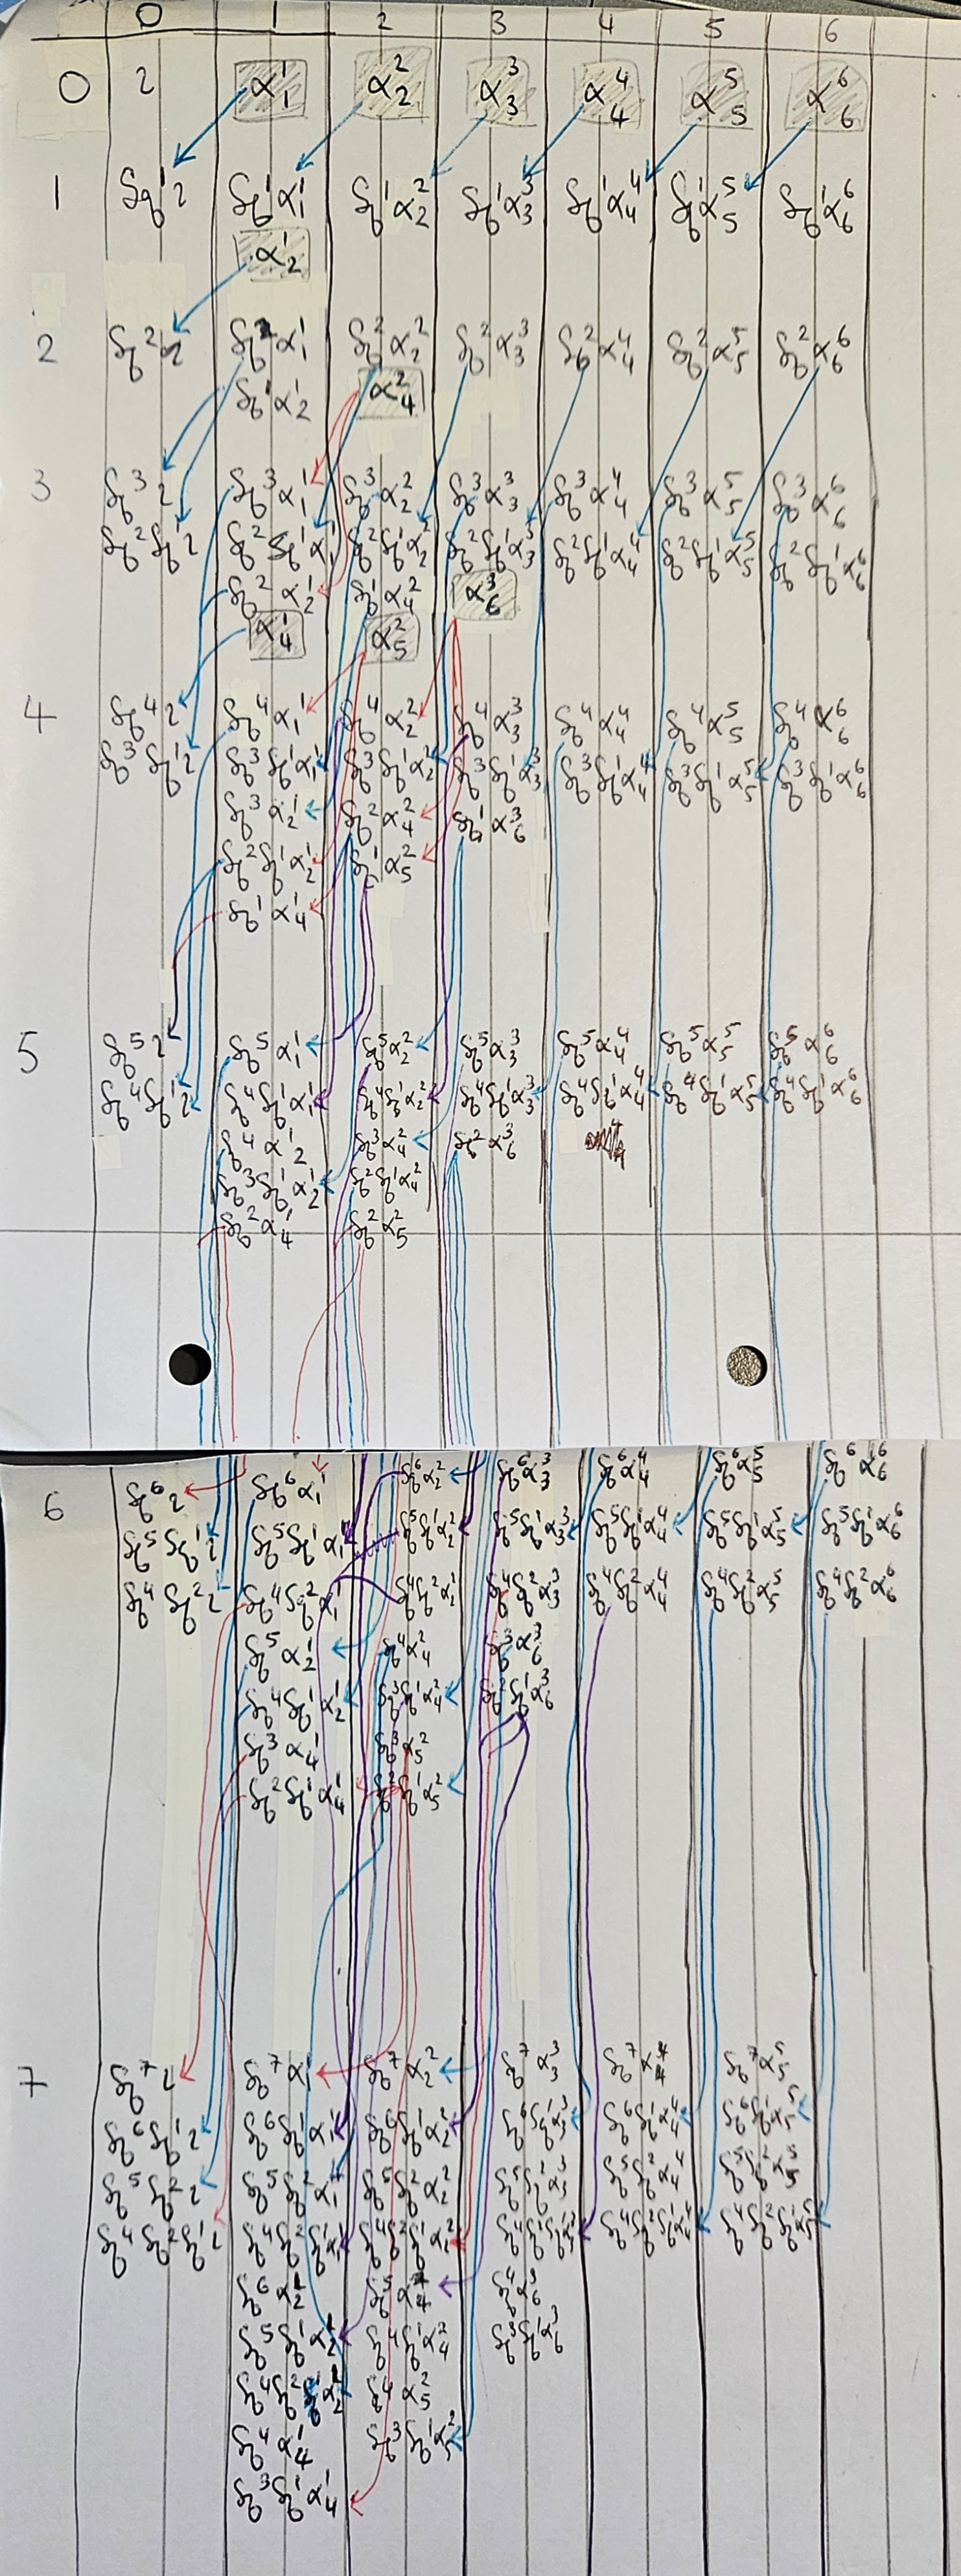
\includegraphics[width=0.4\textwidth]{ext3}
\caption{Calculating the first 5 rows}
\end{figure}

\begin{lemma}[?]
There are no nontrivial differentials for \(t-s\leq 13\). 
\end{lemma}

[Should follow from the Leibniz rule, but we need the multiplicative structure first]

\subsection{Resolving extensions}

[Note: there is a multiplicative structure on the \(E_2\) page of the spectral sequence, which Hatcher says is there and then proceeds to never ever mention again. So I'll have to find another source for this bit. It should correspond to the composition product on \(\pi_*^S\), i.e. given \([f]\in \pi_i^S\), \([g]\in \pi_j^S\), we have \([f][g]=[g \circ \Sigma^j f]\in \pi_{i+j}^S\).

\autocite{ass}, in particular 6.1 and 6.2.

Also, \autocite{spectral_sequences} has some cryptic remarks on p424 and p407 about this but doesn't actually really explain it, and in particular doesn't explain how you could know that some stable homotopy group \textit{isn't} cyclic (e.g. \(\pi_8^S\)).

Some slightly less cryptic comments are made in \autocite{cobordism}, in particular stemming from Lemma 3.1.3. If I just believe this lemma for the moment, assuming its \(a_0\) is the same as my \(\alpha^1_1\), and further believe the calculations done in \autocite{ass} in 6.2, then (I think!) this solves my problems.]

\begin{proposition}[{\autocite{ass}, Cor 6.5}]
We have the following relations:
\begin{align*}
\alpha^i_i &= (\alpha_1^1)^i\\
\alpha_4^2&=(\alpha^1_2)^2\\
\alpha^2_5&=\alpha^1_1 \alpha^1_4\\
\alpha^3_6&=(\alpha^1_1)^2 \alpha_4^1=(\alpha^1_2)^3.
\end{align*}
\end{proposition}

\begin{proposition}[{\autocite{cobordism}, Lem 3.1.3(b)}]
If \(x \in \Ext^{s,t}(\bb{F}_2, \bb{F}_2)\) is a permanent cycle in the Adams spectral sequence represented by \(\alpha \in \pi_*^S\), then \(\alpha^1_1x\) is a permanent cycle represented by \(2 \alpha\). 
\end{proposition}

\begin{theorem}
\begin{align*}
\text{}_{(2)}\pi_i^S = \begin{cases}
\inte/2\inte & i = 1, 2\\
\inte/8\inte & i = 3\\
0 & i = 4, 5.
\end{cases}
\end{align*}
\end{theorem}

\subsection{Nontrivial differentials}

[The point here is that all differentials interacting with \(E^{s,t}\) for \(t-s=14\) are trivial, and thus computing the stable homotopy groups is purely mechanical, because everything that appears on this part of the \(E_2\) page has to survive to \(E_\infty\). Thus, the `ambiguity' at \(t-s=14\) is just the fact that this is the first time you need to actually compute differentials.

For \(t-s<14\) there are only actually the ones emanating from \(E^{1, 2}\) and the \(d_2\) differential starting at \(E^{2, 10}\) to worry about, because all the others either enter or leave \(0\).]

\begin{enumerate}
\item Differentials emanating from \(E^{1, 2}_r\) are trivial: \(0=d_r(h_0h_1)=d_r(h_0)h_1\pm h_0d_r(h_1)=\pm h_0d_r(h_1)\). So \(d_r(h_1)=0\).
\item The \(d_2\) differential at \(E^{2, 10}_2\) is trivial: \(E^{2,10}\) is generated by \(h_1h_3\) (check), and \(d_2(h_1h_3)=d_2(h_1)h_3\pm h_1d_2(h_3)=0+0=0\) (the first one we just checked, the second goes into a zero box).
\item The \(d_2\) differential at \(E^{1, 16}_2\) is nontrivial: \autocite{rognes2}, Thm 11.10.2.
\item The \(d_3\) differential at \(E^{2, 17}_3\) is nontrivial: \autocite{rognes2}, Thm 11.10.7 (which he doesn't prove, so really it's \autocite{rognes2} Table 14.2 (10), which uses a differential \(d_2\) of \(E_2(C\sigma)\) which is on table 14.9 (4)(!)). 
\end{enumerate}

\autocite{stable_homotopy}, \autocite{cobordism}, \autocite{ass}, \autocite{rognes2}.

\appendix 

\section{Algebra}

\subsection{Free resolutions}\label{2502220958}

\begin{definition}
Let \(M, N\) be modules over a ring \(R\). A \textit{resolution} \(F\) of \(M\) is an exact sequence 
\[\cdots \to F_2 \to F_1 \to F_0 \to M \to 0.\]
If in addition each \(F_i\) is a free \(R\)-module, then the resolution is called \textit{free}. 
\end{definition}

Given a free resolution as above, applying \(\Hom_R(-, N)\) gives us a chain complex
\[\cdots \leftarrow \Hom_R(F_2, N) \leftarrow \Hom_R(F_1, N) \leftarrow \Hom_R(F_0, N) \leftarrow \Hom_R(M, N) \leftarrow 0.\]
Dropping the term \(\Hom_R(M, N)\) [why?] we get the sequence
\[\cdots \leftarrow \Hom_R(F_2, N) \leftarrow \Hom_R(F_1, N) \leftarrow \Hom_R(F_0, N) \leftarrow 0,\]
and we define \(\Ext^n_R(M, N)\) to be the \(n\)th homology group of this chain complex. 

%we write \(H^n(F; G):=\ker f^*_{n+1}/\im f_n^*\). Any abelian group \(H\) has a free resolution of the form 
%\[0 \to F_1 \to F_0 \to H \to 0\]
%(the one you think it is). So we get a chain complex
%\[0 \leftarrow F_1^* \leftarrow F_0^* \leftarrow H^* \leftarrow 0.\]
%We have \(H^n(F; G)=0\) for \(n>1\). Define \(\Ext(H;G):=H^1(F;G)\). 

[these do not depend on the choice of free resolution of \(M\)]

A free resolution is \textit{minimal} if at each stage of its construction we choose the minimal number of free generators for \(F_i\) in each degree.

[The above definition is bad but I'm keeping it just for the moment.]

\section{Topology}

All from \autocite{hatcher} unless otherwise stated.

\subsection{Suspension}

\begin{definition}
Let \(X\) be a topological space. The \textit{suspension} \(SX\) is the space \newline\((X\times I)/\sim\), where \((x, 0)\sim (x', 0)\) and \((x,1)\sim (x',1)\) for all \(x,x'\in X\). 
\end{definition}

\begin{definition}
Let \(X\) be a pointed topological space. The \textit{reduced suspension} \(\Sigma X\) is the space \(SX/\sim\), where \([x_0, t]\sim [x_0, t']\) for all \(t,t'\in I\). 
\end{definition}

Given a map \(f : X \to Y\), we can define \(\Sigma f : \Sigma X \to \Sigma Y\) by \(\Sigma f[(x, t)]=[(fx, t)]\). This makes \(\Sigma \) into a functor \(\Sigma : \textbf{Top}\to \textbf{Top}\). 

\begin{remark}\label{2502141442}
\(\Sigma\) is faithful, since for any maps \(f, g : X\to Y\), if \(\Sigma f = \Sigma g\) then in particular \([(fx, \frac{1}{2})]=[(gx, \frac{1}{2})]\), so \(fx=gx\). 
\end{remark}  

[below is reconstructed from  \autocite{mazelgee}]

Given pointed maps \(f, g : \Sigma X \to Z\), define 
\begin{align*}
f \star g : \Sigma X &\to Z\\
[x,t]&\mapsto \begin{cases}
f[x,2t-1] & t \geq \frac{1}{2},\\
g[x,2t] &t\leq \frac{1}{2}.
\end{cases}
\end{align*}
This is well defined, since both \(f\) and \(g\) are basepoint-preserving. %\(f[x,0]=f[x_0,0]=y_0=g[x_0,1]=g[x,1]\). Essentially, it's just because the maps are basepoint-preserving, and \([x,0]\) and \([x,1]\) are both just the basepoint.

\begin{remark}
This defines a group structure on \([\Sigma X, Z]\), and thus \([\Sigma^i X, Z]\) is a group for all \(i\geq 1\). For \(i\geq 2\), these can be shown to be abelian, via the Eckmann-Hilton argument.
\end{remark}

\begin{remark}\label{2502200937}
The homotopy groups \(\pi_i(Z)\) are a special case of the above construction, taking \(X:=S^{i-1}\). 
\end{remark}

%[There are two possible products on \([\Sigma^2 X, Z]\), and some variation on the Eckmann–Hilton argument works its magic to show it's actually commutative (and, apparently, automatically associative). ]

\begin{itemize}
\item Loops; the adjunction \(\Sigma \dashv \Omega\), where \(\Omega\) is the loop functor.
\end{itemize}

\autocite{hatcher}, p395:

\begin{remark}
It follows that \(\pi_{n+1}(X)\cong \pi_n(\Omega X)\). In particular, \(\Omega K(G, n)\) is a \newline\(K(G, n-1)\). 
\end{remark}

\begin{itemize}
\item \autocite{hatcher} 2.1 Ex 20 and 2.2 Ex 32: \(\tilde H_n(X)\cong \tilde H_{n+1}(SX)\), where \(S\) is the (non-reduced) suspension.  (MV?) 
\item Hatcher also says on p219 that \(\tilde H^n(X;R)\cong \tilde H^{n+k}(\Sigma^kX;R)\), where \(\Sigma \) is reduced suspension.
\end{itemize}

\subsection{Other basic constructions}

\begin{definition}
Let \((X, x_0), (Y, y_0)\) be pointed topological spaces, and consider their product \(X\times Y\). The subspaces \(X\times\{y_0\}\cong X\) and \(\{x_0\}\times Y\cong Y\) intersect at exactly one point, \((x_0, y_0)\), and so can be identified with the wedge \(X\vee Y\). We thus define the \textit{smash product} \(X\wedge Y:=(X\times Y)/(X\vee Y)\), with the canonical basepoint \((x_0,y_0)\).  
\end{definition}

\begin{example}
We have \(S^n \wedge S^m\cong S^{n+m}\). [is this obvious?]
\end{example}

\begin{remark}
Note that \(\Sigma X \cong X\wedge S^1\). 
\end{remark}

\begin{remark}
Observe that \(X\wedge (Y\wedge Z)\cong (X\wedge Y)\wedge Z\). Combining this with the remarks above, we see that \(\Sigma^kX=X\wedge S^k\). 
\end{remark}

\begin{remark}\label{2502211505}
Note that \(\Sigma(X\vee Y)\cong \Sigma X\vee \Sigma Y\).
\end{remark}

\begin{itemize}
\item The Eilenberg-MacLane space is \(K(G, n)\), and it has the property that 
\[\pi_i(K(G, n))=\begin{cases}
G & i=n,\\
0 & i\neq n.
\end{cases}\]
They're unique up to weak homotopy equivalence (i.e. if you have another one \(X\), there's a map between them which descends to an isomorphism on homotopy groups). They can be taken to be CW complexes. 
\end{itemize}

\begin{definition}
Let \(X\), \(Y\) be topological spaces, where \(X\) has a basepoint \(x_0\). Then the \textit{reduced product} \(X\times_{\text{red}}Y:=(X\times Y)/(x_0 \times Y)\). 
\end{definition}

\begin{definition}
Let \(f : X \to Y\) be a map. The \textit{mapping cylinder} \(M_f\) is defined by \((X\times I)\sqcup Y/\sim\), where \((x,1)\sim f(x)\) for all \(x \in X\). 
\end{definition}

The mapping cylinder deformation retracts onto \(Y\) via \(h : M_f \times I\to M_f\); \(([x,t], s)\mapsto [x, t+s(1-t)]\). If \((X, x_0), (Y, y_0)\) are pointed spaces, the \textit{reduced mapping cylinder} is the quotient \(M_f/\sim\), where \([x_0, t]\sim [x_0, t']\) for all \( t\in I\).

\begin{definition}
Let \(f : X \to Y\) be a map. The \textit{mapping cone}\footnote{Why does Hatcher not insist this guy is reduced, like he does with the mapping cylinders?} \(C_f\) is defined to be \(Y\sqcup_f CX:=(Y\sqcup CX)/(f(x)\sim [x,1])\). 
\end{definition}

\subsection{Cell complexes}\label{2502141508}

\begin{definition}
Let \(X\) be a cell complex, \(A\subq X\) a subcomplex. Then the quotient \(X/A\) has a cell complex structure, with cells the cells of \(X\setminus A\) along with a basepoint (the image of \(A\) in \(X\)). 
\end{definition}

\begin{definition}
Let \(f : X \to Y\) be a map between CW complexes. Then \(f\) is \textit{cellular} if \(f(X_{(n)})\subq Y_{(n)}\) for all \(n\), where \(X_{(n)}\) is the \(n\)-skeleton of \(X\). 
\end{definition}

Cellular approximation theorem:

%might not even need this but it looks useful
\begin{theorem}[{\autocite{hatcher}, Thm 4.8}]\label{2502211420}
Let \(f : X \to Y\) be a map of CW complexes. Then \(f\) is homotopic to a cellular map.
\end{theorem}

\begin{lemma}[{\autocite{hatcher}, Prop 0.16}]\label{2502211419}
Let \(A\subq X\) be CW complexes. Then the pair \((X, A)\) has the \textit{homotopy extension property}; that is, for any map \(f : X \to Y\) and homotopy \(h : A\times I \to Y\) such that \(h(a,0)=f|_A\), there is a homotopy \(\tilde h : X\times I \to Y\) extending \(h\). 
\end{lemma}

\begin{itemize}
\item The product of cell complexes is a cell complex (maybe only if one of them is finite?)
\item The smash product of (pointed?) cell complexes is a cell complex (maybe only if one is them is finite?) [\autocite{hatcher} says ``the smash product \(X\wedge Y\) is a cell complex if \(X\) and \(Y\) are cell complexes with \(x_0\) and \(y_0\) \(0\)-cells, assuming that we give \(X\times Y\) the cell-complex topology rather than the product topology in cases where these two topologies differ''.]
%\item The reduced suspension of a pointed cell complex is a pointed cell complex.
%\item CW pairs? [they're literally just pairs of some CW complex and a subcomplex]
\item For a CW complex \(X\), \(SX\simeq \Sigma X\).
\item The reduced suspension of a pointed cell complex \((X, x_0)\) is another pointed cell complex \(\Sigma X\) with basepoint \(x_0\) and an \(n\)-cell for each non-basepoint \(n-1\) cell \(e^{n-1}_\alpha\) of \(X\).
\end{itemize}

\begin{definition}
Let \(X\) is a topological space. A \textit{CW approximation} to \(X\) is a CW complex \(Z\) equipped with a weak homotopy equivalence \(f : Z \to X\).
\end{definition}

\begin{theorem}[{\autocite{hatcher}, Prop 4.13}]
Every space \(X\) has a CW approximation \(f : Z \to X\). %If \(X\) is path-connected, \(Z\) can be chosen to have a single 0-cell, with all other cells attached by basepoint-preserving maps. 
\end{theorem}

\begin{itemize}
\item In particular, \(\Omega K(G, n)\) has a CW approximation \(Z \to \Omega K(G, n)\), and since \(\Omega K(G,n)\) is a \(K(G,n-1)\), so is \(Z\). 
\item Something along the lines of `compact \(\leftrightarrow\) finite number of cells'.
\end{itemize}

\section{Notes to self}\label{C}

\subsection{Vague problems and Questions}

\begin{itemize}
%\item Is `pointed' (co)homology just reduced (co)homology? I've noticed `pointed things' (\(\Sigma, \Omega, \wedge\), ...) seem to happen to/in reduced (co)homology, and `unpointed things' (\(S, \times, ...\)) happen to/in normal (co)homology. I want to do pointed things. 

%\item \autocite{hatcher} says that defining cohomology of a spectrum as just \(\colim_n H^{i+n}(X_n)\) in the same way as for homotopy works for EM spectra and suspension spectra

\item What does Hatcher mean when he says two spectra are `equivalent'?

\item On p588 of \autocite{hatcher5}, he says ``every CW spectrum is equivalent to a suspension spectrum''. Does he actually mean that, or does he mean `equivalent to the suspension of a spectrum'? The former seems way too strong, although in fairness I still don't know what an equivalence of spectra actually \textit{is}. 

%\item Suppose I have the \(E_2\) page for the appropriate spectral sequence. That in principle only gives me the `dots' and possibly the differentials. But if I just want to calculate, say, \(\pi^S_3\), I get \(\inte_2\) summands at \(E^{1, 4}_2, E^{2, 5}_2,\) and \(E^{3, 6}_2\). So, that says I have a filtration 
%\[0 \subq \inte_2 \subq F^{2,5}\subq F^{1,4}=\pi^S_3,\]
%and \(F^{2,5}/\inte_2\cong \inte_2\), \(F^{1,4}/F^{2,5}\cong \inte_2\). So \(\pi^S_3\) has order 8 and a filtration by \(\inte_2\)'s, but that still doesn't tell me whether it's \(\inte_8, \inte_4\times \inte_2\) or \(\inte_2^3\)? Thm 5.47 of \autocite{hatcher5} tells me that \(F^{s,t}\) is the image of the map \(\pi_t(\bb{S}_s)\to \pi_3^S\), so do I have to go back to the constructing and figure out what that map actually is, or is there something algebraic I can do?\footnote{I think this related to something \autocite{ass} calls the Yoneda product on p47-50 and 61-62 - this is a multiplicative structure on \(E_2\) and should tell me something about the additive structure of \(\pi_*^S\).}
\item Replacing maps by inclusions?
\item I am definitely being told some lies about what the spectral sequence actually converges to. There's a strong implication/actual statement(!!) that at each \(i\) it's supposed to be a filtration of \(\pi_i^S\) modulo odd torsion, but I think this isn't true. I think it's actually the 2-completion\footnote{Whatever that means.} of \(\pi_i^S\). That coincides with the \(p\)-primary part for finite abelian groups, but for \(\pi_0^S\) it's supposed to be \(\inte_2\) (i.e. the 2-adic integers), not \(\inte\). I believe. Maybe get a source for this. Some people say it's the localisation at 2?? But I think that's also a lie. 
\item The Leibniz rule is \(d_r(xy)=d_r(x)y\pm xd_r(y)\) (can't remember the sign). But anything I'm using that rule on is some generator of an \(\bb{F}_2\), right? So the sign shouldn't matter. But then, shouldn't the Yoneda product be graded commutative (and thus commutative, because again, in the target signs don't matter)? So why does \autocite{ass} have some comment (to find later) about how the Yoneda product is commutative ``in some range''?? 

\end{itemize}

\subsection{To do}

Now:

\begin{itemize}
\item The definition of Ext in \ref{2502220958} has only one superscript, but the Ext in the Adams spectral sequence has a bigrading - figure out where the extra index came from and write it down so I don't forget it.
\item Read about fibration and cofibration sequences of CW complexes. 
\item Find out what a (co)homology theory is. 
\item Find out what the deal with reduced cohomology and being stable under suspension is.
\item Apparently it's not difficult to show that for \(i\geq 1\), \(\pi_i^S\) is finite? I should show this so I don't have to worry about all this completion business. 
\end{itemize}

Eventually:

\begin{itemize}
\item Be consistent with either cell complex or CW complex (eventually)
\item Be consistent with \(\bb{F}_2\)  or \(\inte/2\inte\) (don't use \(\inte_2\), that's really bad).
\item Specialise the Adams spectral sequence (i.e. set \(Y=\bb{S}\)).
\item Remember that you have to hand in the tex file, so for the love of god change anything stupid that's hidden in the pdf.
\item Sometimes I say \(\pi_*^S\) or \(\text{}_{(2)}\pi_*^S\) (localised at 2?) instead of its completion at 2 or whatever. So make sure it's correct.
\item Stick to a convention on suspension/cone/homotopy numbering. I.e. Does a homotopy start at 0 or 1? Does a suspension go from -1 to 1 with the space in the middle at 0, or 0 to 1 with the space at \(1/2\)? Do cones go from 0 to 1, and if so, make sure when they include into suspensions they do so consistently. 

\end{itemize}

\subsection{Other notes}

\begin{itemize}
\item READ IF YOUR CALCULATIONS AREN'T WORKING: You are working modulo 2!!!
%\item There are two ways I can play the chapter on spectra. The first is to constantly draw analogues with CW complexes, carry over all the theorems and prove them in a similar way, really emphasising that these are the `stable' versions of CW complexes and we should definitely think about them that way. The other is really stupid I just realised so I'll just do the first thing I said. 
\item If you have a bunch of maps between graded modules/algebras, they're graded homomorphisms. So they preserve degree. 
\item All (co)homology is supposed to be reduced.
\item On p592 of \autocite{hatcher5}, he says that ``for spectra \(X\) of finite type [the more general] definition of an \(\A\)-module structure on \(H^*(X)\) agrees with the definition using the usual \(\A\)-module structure on the cohomology of spaces and the identification of \(H^*(X)\) with the inverse limit \(\lim\limits_{\leftarrow}H^{*+n}(X_n)\)''. Absolutely everything relevant to spheres in the construction of the Adams spectral sequence seems to only use spectra of finite type, but Hatcher says on p585 that we can't just take the inverse limit because it doesn't work for the `more general spectra' used when constructing the Adams spectral sequence. I believe this is because the Adams spectral sequence is defined for \(X\) not of finite type, though Hatcher only constructs it for finite type guys.
\item Signs don't matter with the Leibniz rule either!! You are working modulo 2!!!!!!!!
\item Remember, once you know that \(d_2(h_4)=h_0h_3^2\), you know \(h_4\) \textit{doesn't survive to the third page}. So, for example, \(d_3(h_0h_4)\neq h_0d_3(h_4)\) because \(h_4\) doesn't exist anymore. That's why \(d_3(h_0h_4)\) can be nonzero. 
\item As previously mentioned, we are working modulo 2!! What this also implies is that if anything is hit by any sort of differential, or has any nonzero differential coming out of it, it's completely killed by the next page. Because the summands are just a bunch of \(\bb{F}_2\)'s (so you don't need to worry about `how much' of something is killed, it all is). 
\end{itemize}

\printbibliography

\end{document}